\documentclass[12pt,letter]{article}
\usepackage[moduleName=S-SMP(Echo)]{KautenjaDSP}
% import a debugging package to show the margin boxes
% \usepackage{showframe}
% set the graphics path to the img directory
\graphicspath{{img/}}

% algorithm2e stuff
% \SetKwInOut{Objects}{$\CKmatrix{O}$}
% \SetKwInOut{Weights}{$\CKvector{w}$}

\begin{document}
\titlePage{S-SMP-Echo-Logo}{S-SMP-Echo-Module}{KautenjaDSP}

% -------------------
% MARK: Overview
% -------------------

\section{Overview}

\begin{figure}[!htp]
\centering
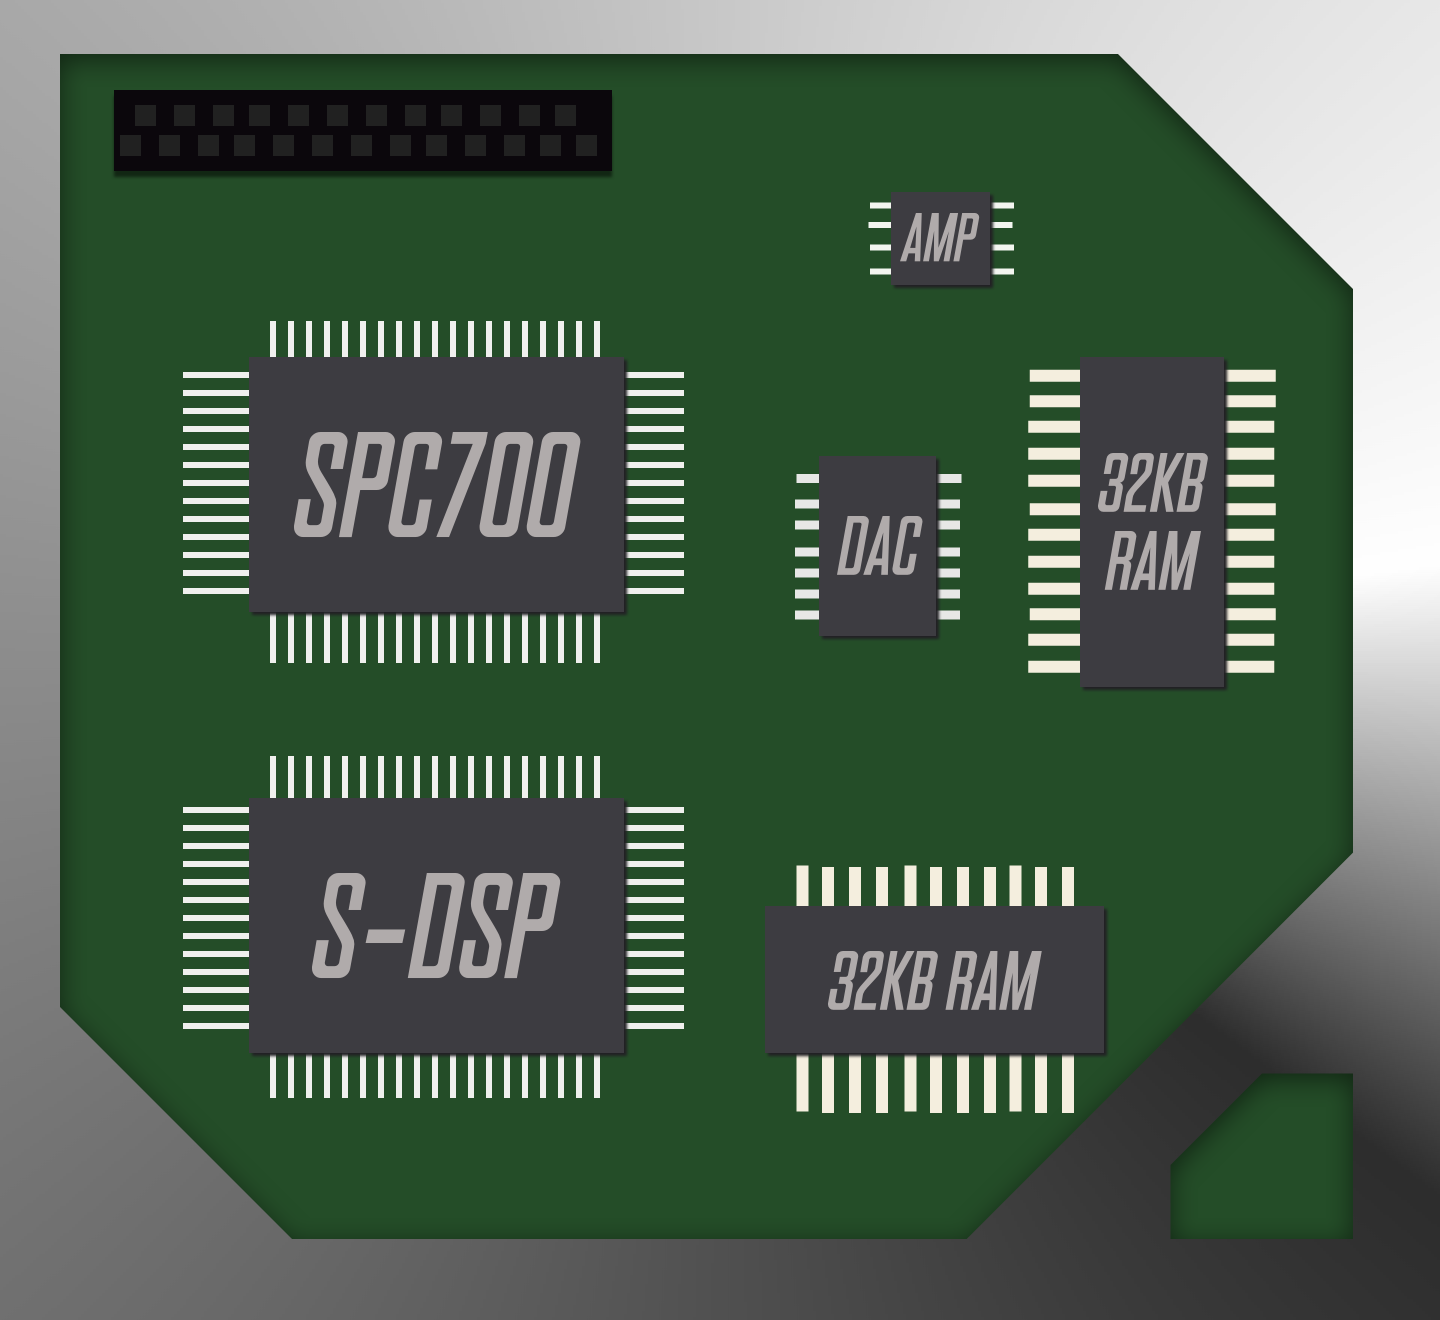
\includegraphics[width=0.5\textwidth]{S-SMP-Chip}
\caption{The S-SMP module from the SNES. The S-SMP included two discrete microprocessors: the SPC700, and the S-DSP. The SPC700 performed primary computation, while the S-DSP performed DSP specific computations, like BRR decoding, sample playback, applying the echo effect, mixing levels, etc. The SPC700 and S-DSP shared $64KB$ of total RAM that was used for BRR sample data and the echo buffer. The digital audio is decoded back to an analog signal by a 16-bit DAC and amplified using an Op-Amp. Before digital-to-analog conversion, the output audio is low-pass filtered by a Gaussian filter that gives the S-SMP chip a distinctive sound.}
\end{figure}

\clearpage

S-SMP(Echo) is a Eurorack module that emulates the echo effect from the S-SMP sound chip on the Super Nintendo Entertainment System (SNES). The Echo effect of the S-SMP chip has $15$ different delay levels of $16ms$ each, a $64KB$ echo buffer, an 8-tap FIR filter for shaping the sound of the echo, parameterized feedback, and parameterized dry / wet mix level. The echo buffer is stereo, although the echo parameters and coefficients of the FIR filter are the same for both channels.

S-SMP(Echo) provides the key features of the echo module of the S-SMP chip,
namely,
\begin{itemize}
  \item \textbf{$32KHz$ Sample Rate:} The S-SMP was designed to run at $32kHz$, so the audio inputs and outputs of the module are locked to $32kHz$.
  \item \textbf{Stereo Echo Buffer:} Echo buffer for two independent inputs in stereo configuration. The parameters are the same for both inputs, but the inputs have their own dedicated echo buffers.
  \item \textbf{Expanded Delay:} The 15 levels of delay has been upgraded to 31 levels that each add an additional $16ms$ of delay (up to roughly $500ms$). 31 levels of delay is able to fit in the RAM of the original S-SMP, but the instruction set does not normally support the addressing of 31 levels.
  \item \textbf{Feedback:} Additive and subtractive feedback following the original implementation
  \item \textbf{Surround Effect:} Stereo mixer with the ability to invert the phase of either channel resulting in odd Haas effects.
  \item \textbf{8-tap FIR Filter:} Fully parameterized 8-tap FIR filter for shaping the sound of the echo. The filter can be parameterized as low-pass, high-pass, band-pass, band-stop, etc. and includes presets with filter parameters from popular SNES games.
  \item \textbf{16-bit Inputs:} The BRR decoder has been remove in this emulation. Instead, input audio is sampled directly as 16-bit PCM. A separate module S-SMP(BRR) can be cascaded into S-SMP(Echo) to introduce authentic BRR down-sampling effects to the signal path.
  \item \textbf{Gaussian Low-Pass Filter Override:} The Gaussian low-pass filter has been removed in this emulation. A separate module, S-SMP(Gaussian), can be used in cascade with S-SMP(Echo) to produce a more authentic SNES sound.
\end{itemize}

% -------------------
% MARK: Panel Layout
% -------------------

\clearpage
\section{Panel Layout}

\begin{figure}[!htp]
\centering
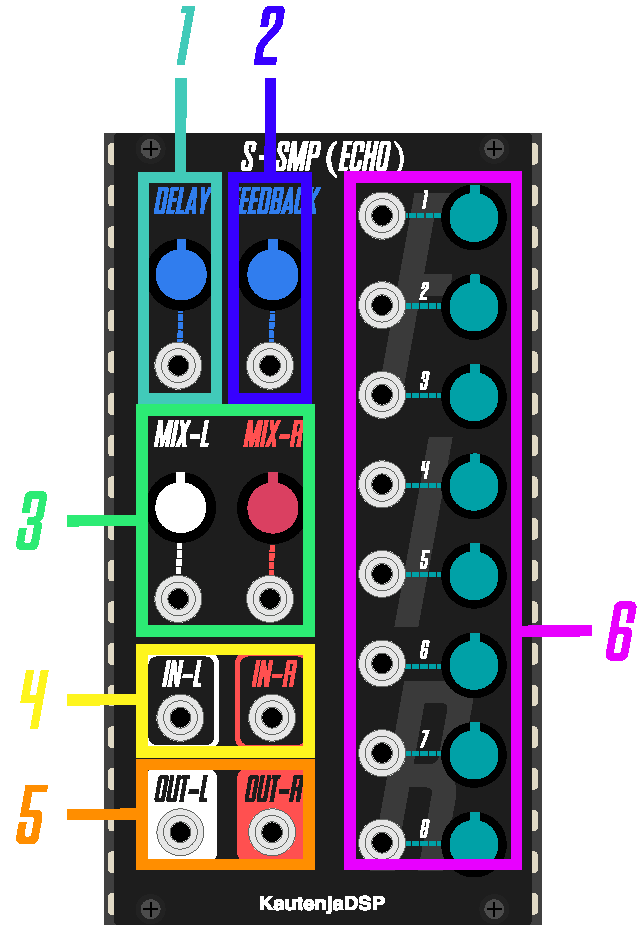
\includegraphics{S-SMP-Echo-Manual}
\end{figure}

\clearpage
\begin{enumerate}
  \item TODO
\end{enumerate}

% -------------------
% MARK: References
% -------------------

\clearpage
\renewcommand\refname{References \& Acknowledgments}
\nocite{*}
\bibliographystyle{apalike}
\bibliography{references}

\end{document}
